\section{Complex numbers}

From the section \hyperref[sec:equations]{Equations} we saw that if the discriminant of a quadratic equation is negative, the
equation has no real solution. For example, the equation $$x^2+4=0$$ has no real solution. If we try to solve this equation, we get $x^2=-4$, so $$x=\pm \sqrt{-4}$$
But this is impossible, since the square of any real number is positive. [For example, $(-2)^2=4$, a positive number.] Thus negative numbers don’t have real square roots.
To make it possible to solve all quadratic equations, mathematicians invented an
expanded number system, called the complex number system. First they defined the new
number $i$ which is, $$i=\sqrt{-1}$$ This means that $i^2=-1$. A complex number is then a number of the form $a+bi$, where $a$ and $b$ are real numbers. 

\begin{align*}
    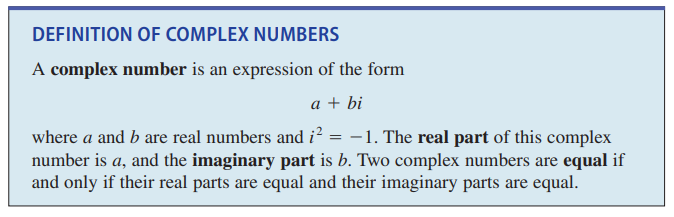
\includegraphics[width=1.1\textwidth]{algebra-pre-calculus/complex-numbers/complex_numbers_def.png}
\end{align*}

In the complex number the reason why $b$ is being called as the \textbf{imaginary part} is not because it's an imaginary number(when squared produce negative outcome). It's because it's being multiplied by the imaginary number $i$, so it's kind of the "part" of it. The real part is the part that is \textbf{not} being multiplied by $i$. \\

Note that both the real and the imaginary part are real numbers. 

A number such as $6i$, which has real part 0, is called a \textbf{pure imaginary number}. A
real number such as $-7$ can be thought of as a complex number with imaginary part 0.
In the complex number system every quadratic equation has solutions. The numbers
$2i$ and $-2i$ are solutions of $x^2-4$ because

\begin{align*}
    (2i)^2&=4i^2=-4 \\
    (-2i)^2&=4i^2=-4
\end{align*}

We study complex numbers because they complete, in a useful and elegant
fashion, our study of the solutions of equations. In fact, imaginary numbers are useful not
only in algebra and mathematics, but in the other sciences as well. To give just one example, in electrical theory the reactance of a circuit is a quantity whose measure is an
imaginary number. \\

\subsection{Arithmetic Operations on Complex Numbers}

Complex numbers are added, subtracted, multiplied, and divided just as we would any
number of the form $a+b\sqrt{c}$. The only difference that we need to keep in mind is that $i^2=-1$. Thus the following calculations are valid.

\begin{align*}
    (a+bi)(c+di)&= ac+adi+bci+bdi^2 \\
    &=ac+(ad+bc)i-bd \\
    &= (ac-bd)+(ad+bc)i
\end{align*}

\begin{align*}
    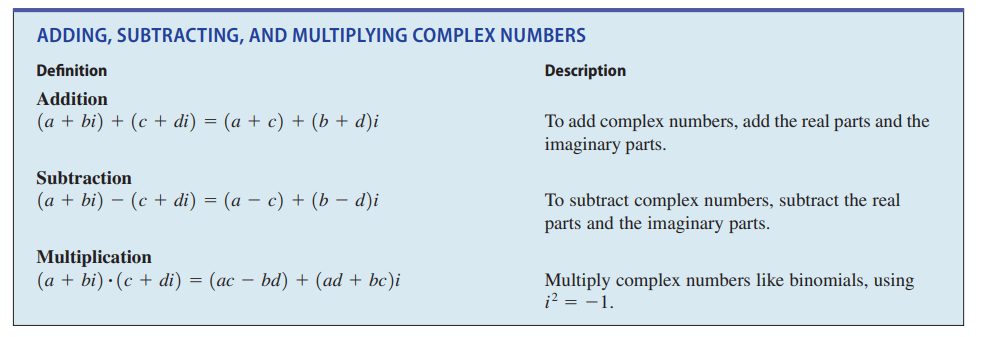
\includegraphics[width=1.1\textwidth]{algebra-pre-calculus/complex-numbers/arithmetic_operations_complex_numbers.png}
\end{align*}

\subsection{Examples of Adding and subtracting complex numbers}
\textbf{(a)} $(3+5i)+(4-2i)=(3+4)+(5-2)i=7+3i$